%% GRAFT Presentation — 15 min talk
%% Compile with: pdflatex graft_presentation.tex
%%
\documentclass[aspectratio=169,12pt]{beamer}

%% ── Theme ───────────────────────────────────────────────────────────────────
\usetheme{metropolis}
\usepackage{appendixnumberbeamer}

%% ── Packages ────────────────────────────────────────────────────────────────
\usepackage[utf8]{inputenc}
\usepackage[T1]{fontenc}
\usepackage{booktabs}
\usepackage{amsmath}
\usepackage{amssymb}
\usepackage{graphicx}
\usepackage{multirow}
\usepackage{xcolor}
\usepackage{tikz}
\usepackage{array}
\usepackage{caption}
\usepackage{hyperref}

%% ── Custom Colours ──────────────────────────────────────────────────────────
\definecolor{accent}{HTML}{2563EB}       % Blue accent
\definecolor{positive}{HTML}{16A34A}     % Green for improvements
\definecolor{negative}{HTML}{DC2626}     % Red for regressions
\definecolor{muted}{HTML}{6B7280}        % Grey for secondary text
\definecolor{highlight}{HTML}{F59E0B}    % Amber for emphasis

\setbeamercolor{frametitle}{bg=accent!10, fg=accent!90!black}
\setbeamercolor{progress bar}{fg=accent}
\setbeamercolor{alerted text}{fg=accent}

%% ── Macros ──────────────────────────────────────────────────────────────────
\newcommand{\pg}{\textsc{pg}}
\newcommand{\plus}[1]{{\color{positive}+#1}}
\newcommand{\minus}[1]{{\color{negative}$-$#1}}
\newcommand{\mhuman}{M\textsubscript{human}}
\newcommand{\mauto}{M\textsubscript{auto}}
\newcommand{\mcpg}{M\textsubscript{cpg}}

%% ── Title ───────────────────────────────────────────────────────────────────
\title{\textbf{GRAFT}:\\Grounding Region Annotations into\\Fine-Tuned Transformers}
\subtitle{TTIC 31280 — Models for Representing Images \& Videos}
\author{Siddharth Raj \and Aniket Agrawal}
\institute{University of Chicago}
\date{Spring 2026}

\begin{document}

%% ═══════════════════════════════════════════════════════════════════════════
%% TITLE
%% ═══════════════════════════════════════════════════════════════════════════
\begin{frame}[plain]
  \maketitle
\end{frame}

%% ═══════════════════════════════════════════════════════════════════════════
%% PART 1: MOTIVATION & SETUP  (~5 min)
%% ═══════════════════════════════════════════════════════════════════════════
\begin{frame}{Outline}
  \tableofcontents
\end{frame}

\section{Motivation \& Setup}

%% ─── Slide 1: The Problem ──────────────────────────────────────────────────
\begin{frame}{The Problem: Spatial Blindness in VLMs}
  \begin{columns}[T]
    \begin{column}{0.55\textwidth}
      \textbf{Vision-language models} (CLIP, SigLIP) are trained with\\
      \alert{global image--text contrastive objectives.}
      \vspace{0.5em}

      Patch tokens know \textbf{what} is in the image,\\
      but not \textbf{where}.

      \vspace{1em}
      \textbf{Why does this matter?}
      \begin{itemize}
        \item Referring expression comprehension
        \item Dense captioning
        \item Any spatial reasoning about language
      \end{itemize}
    \end{column}
    \begin{column}{0.42\textwidth}
      \begin{center}
        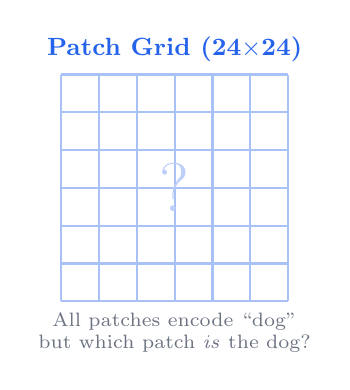
\begin{tikzpicture}[scale=0.8]
          % Image patch grid
          \draw[step=0.6, thick, accent!40] (0,0) grid (3.6,3.6);
          \node[font=\small\bfseries, accent] at (1.8, 4.0) {Patch Grid (24$\times$24)};

          % Question mark overlay
          \node[font=\Huge, accent!30] at (1.8, 1.8) {?};

          % Label
          \node[font=\scriptsize, muted, text width=3.5cm, align=center] at (1.8, -0.5) {
            All patches encode ``dog''\\but which patch \emph{is} the dog?
          };
        \end{tikzpicture}
      \end{center}
    \end{column}
  \end{columns}
\end{frame}

%% ─── Slide 2: Why SigLIP? ─────────────────────────────────────────────────
\begin{frame}{Why SigLIP?}
  \begin{itemize}
    \item SigLIP uses \alert{sigmoid contrastive loss} (per-pair, no batch denominator)
    \item Produces \textbf{stronger image-text matching} than CLIP
    \item But sigmoid objective has \textbf{even less spatial bias}\\
          \quad — no denominator to encourage patch-level diversity
    \item[$\Rightarrow$] \textbf{Harder test case}: success here implies the approach generalises
  \end{itemize}

  \vspace{1em}
  \begin{block}{Our backbone}
    \texttt{google/siglip-base-patch16-384}\\
    \small 729 patches per image (27 $\times$ 27 grid), $\sim$200M parameters
  \end{block}
\end{frame}

%% ─── Slide 3: What We Do ──────────────────────────────────────────────────
\begin{frame}{GRAFT: What We Built}
  \begin{center}
    \textbf{Freeze SigLIP} $+$ \textbf{LoRA adapters} $+$ \textbf{Region loss}
  \end{center}
  \vspace{0.3em}

  \begin{columns}[T]
    \begin{column}{0.48\textwidth}
      \textbf{Architecture:}
      \begin{itemize}
        \item LoRA on $q$-proj, $v$-proj
        \item Rank 4, $\alpha=16$
        \item \textbf{295K trainable params}\\(0.14\% of backbone)
        \item MaskCLIP bypass on final vision attention layer
      \end{itemize}
    \end{column}
    \begin{column}{0.48\textwidth}
      \textbf{Loss:}
      \begin{equation*}
        \mathcal{L} = \mathcal{L}_{\text{global}} + 0.5 \cdot \mathcal{L}_{\text{region}}
      \end{equation*}
      \begin{itemize}
        \item $\mathcal{L}_{\text{global}}$: sigmoid-SigLIP on\\
              MHAP pooler $\leftrightarrow$ EOS caption
        \item $\mathcal{L}_{\text{region}}$: FILIP-style\\
              EOS phrase $\leftrightarrow$ patch features,\\
              max-pool over in-bbox patches
      \end{itemize}
    \end{column}
  \end{columns}
\end{frame}

%% ─── Slide 4: Data & Eval ──────────────────────────────────────────────────
\begin{frame}{Data \& Evaluation}
  \begin{columns}[T]
    \begin{column}{0.48\textwidth}
      \textbf{Training Data:}
      \begin{itemize}
        \item Flickr30k-Entities (29K images)
        \item Human-annotated phrase $\to$ bbox pairs
        \item $\sim$5.7 phrases/image
        \item Also tested: Florence-2 auto-annotations
      \end{itemize}
    \end{column}
    \begin{column}{0.48\textwidth}
      \textbf{Evaluation:}
      \begin{itemize}
        \item \alert{Pointing Game (PG)}: argmax patch centre inside GT bbox?
        \item 200-image val split (2,124 phrase-bbox pairs)
        \item Held-out test: 2,900 images (28,467 pairs)
        \item \textbf{All results: 3-seed mean $\pm$ std}
      \end{itemize}
    \end{column}
  \end{columns}

  \vspace{1em}
  \begin{block}{Frozen Baseline (B0)}
    PG = \textbf{14.74\%} \quad|\quad
    R@1 top-25 = 7.91\% \quad|\quad
    R@1 halfmax = 7.58\%
  \end{block}
\end{frame}

%% ═══════════════════════════════════════════════════════════════════════════
%% PART 2: MAIN FINDINGS  (~5 min)
%% ═══════════════════════════════════════════════════════════════════════════
\section{Main Findings}

%% ─── Slide 5: Key Insight ──────────────────────────────────────────────────
\begin{frame}{Core Insight: Representation Alignment $>$ Loss Design}
  \begin{center}
    \Large
    The two biggest gains come from\\
    \alert{fixing train/eval mismatches},\\
    not from changing the loss or model.
  \end{center}

  \vspace{1em}
  \begin{enumerate}
    \item \textbf{Image path} (MaskCLIP bypass during training): \plus{7.34 pp}
    \item \textbf{Text path} (EOS token alignment): \plus{2.08 pp}, $6\times$ variance collapse
  \end{enumerate}

  \vspace{0.5em}
  {\small \color{muted} All ablations varying loss weight, LoRA targets, and aggregation returned to the same mean once mismatches were fixed.}
\end{frame}

%% ─── Slide 6: Image-Path Fix ──────────────────────────────────────────────
\begin{frame}{Fix \#1: Image-Path Alignment}
  \begin{columns}[T]
    \begin{column}{0.55\textwidth}
      \textbf{The mismatch:}
      \begin{itemize}
        \item \textbf{Training}: patch features through full self-attention
        \item \textbf{Eval}: MaskCLIP bypass $\rightarrow$ $W_O \cdot W_V \cdot h$\\
              (no inter-patch mixing)
      \end{itemize}

      \vspace{0.5em}
      \textbf{The fix:} Install bypass \emph{before} training.

      \vspace{0.5em}
      \textbf{Effect:}
      \begin{itemize}
        \item Without bypass: PG = 13.42\% \minus{1.32 pp vs B0}
        \item With bypass: PG = 22.08\% \plus{7.34 pp vs B0}
        \item \textbf{One-line change, +8.66 pp swing}
      \end{itemize}
    \end{column}
    \begin{column}{0.42\textwidth}
      \begin{center}
        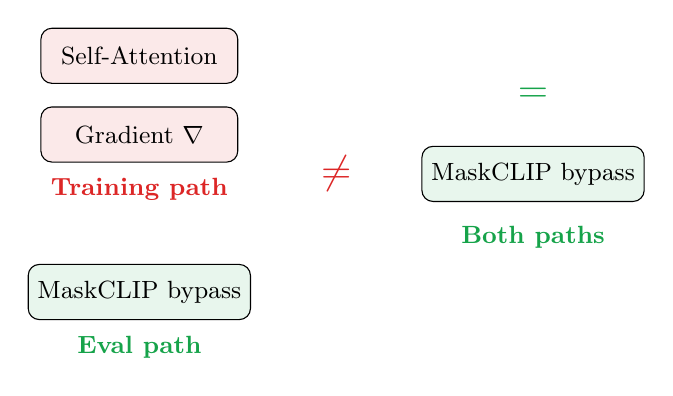
\begin{tikzpicture}[
          box/.style={draw, rounded corners, minimum height=0.7cm, minimum width=2.5cm, font=\small},
          arr/.style={->, thick}
        ]
          % Before
          \node[box, fill=negative!10] (sa) at (0, 3) {Self-Attention};
          \node[box, fill=negative!10] (grad) at (0, 2) {Gradient $\nabla$};
          \node[font=\small\bfseries, negative] at (0, 1.3) {Training path};

          \node[box, fill=positive!10] (mc) at (0, 0) {MaskCLIP bypass};
          \node[font=\small\bfseries, positive] at (0, -0.7) {Eval path};

          \node[font=\Large, negative] at (2.5, 1.5) {$\neq$};

          % After
          \node[box, fill=positive!10] (mc2) at (5, 1.5) {MaskCLIP bypass};
          \node[font=\small\bfseries, positive] at (5, 0.7) {Both paths};
          \node[font=\Large, positive] at (5, 2.5) {$=$};
        \end{tikzpicture}
      \end{center}
    \end{column}
  \end{columns}
\end{frame}

%% ─── Slide 7: Text-Path Fix ───────────────────────────────────────────────
\begin{frame}{Fix \#2: Text-Path Alignment + Variance Collapse}
  \textbf{Same idea, text side:}
  \begin{itemize}
    \item Training used \texttt{mean(hidden\_states)} for phrase embedding
    \item Eval used \texttt{EOS token} (last position)
    \item \textbf{Fix:} Use EOS token everywhere
  \end{itemize}

  \vspace{0.5em}
  \begin{center}
    \begin{tabular}{l c c c}
      \toprule
      & PG (mean $\pm$ std) & Range & $\Delta$ vs B0 \\
      \midrule
      v5 (mean-over-tokens) & 18.68 $\pm$ 2.57\% & [15.87, 20.90] & \plus{3.94} \\
      \textbf{v10 (EOS fix)} & \textbf{20.76 $\pm$ 0.41\%} & [20.48, 21.23] & \textbf{\plus{6.02}} \\
      \bottomrule
    \end{tabular}
  \end{center}

  \vspace{0.5em}
  \begin{center}
    {\Large $\sigma$: 2.57\% $\longrightarrow$ 0.41\% \quad ($\mathbf{6\times}$ reduction)}
  \end{center}
\end{frame}

%% ─── Slide 8: Multi-epoch results ─────────────────────────────────────────
\begin{frame}{Longer Training: Staircase Improvement (v11, 5 epochs)}
  \begin{columns}[T]
    \begin{column}{0.52\textwidth}
      \textbf{Per-epoch cosine restarts:}
      \begin{itemize}
        \item Epochs 1--3: reproduce 1-epoch result ($\sim$19--20\%)
        \item \alert{Epoch 4: step change +3--5 pp}
        \item Epoch 5: plateau at new level
      \end{itemize}

      \vspace{0.5em}
      \textbf{Best result (seed 1):}
      \begin{itemize}
        \item Val PG = \textbf{24.44\%} \plus{9.70 pp vs B0}
        \item Test PG = \textbf{26.16\%} \plus{11.42 pp vs B0}
        \item Test signal: $\sim$48$\sigma$
      \end{itemize}
    \end{column}
    \begin{column}{0.45\textwidth}
      \begin{center}
        \begin{tikzpicture}[scale=0.65]
          % Axes
          \draw[->] (0,0) -- (8,0) node[right] {\small Step};
          \draw[->] (0,0) -- (0,6.5) node[above] {\small Val PG\%};

          % Grid lines
          \foreach \y in {1,2,3,4,5,6} {
            \draw[gray!20] (0,\y) -- (8,\y);
          }

          % Y-axis labels
          \node[left, font=\tiny] at (0,0) {14};
          \node[left, font=\tiny] at (0,1) {16};
          \node[left, font=\tiny] at (0,2) {18};
          \node[left, font=\tiny] at (0,3) {20};
          \node[left, font=\tiny] at (0,5) {24};

          % B0 baseline
          \draw[dashed, muted] (0,0) -- (8,0);
          \node[right, font=\tiny, muted] at (6.5,0.3) {B0=14.74};

          % Trajectory (approximate)
          \draw[thick, accent] (0,0) -- (1,1.2) -- (2,2.7) -- (3,2.9) -- (4,2.5);
          \draw[thick, accent] (4,2.5) -- (4.5,1.7) -- (5,2.4) -- (5.5,2.5) -- (6,2.7);
          \draw[thick, highlight, ultra thick] (6,2.7) -- (6.5,4.5) -- (7,4.8) -- (7.5,5.3) -- (8,5.2);

          % Epoch labels
          \node[below, font=\tiny] at (2, -0.3) {Ep 1--3};
          \node[below, font=\tiny, highlight] at (7, -0.3) {Ep 4--5};

          % Star at peak
          \node[star, star points=5, star point ratio=2.5, fill=highlight, minimum size=4pt] at (7.5, 5.3) {};
          \node[right, font=\tiny, highlight] at (7.7, 5.5) {24.44\%};
        \end{tikzpicture}
      \end{center}
    \end{column}
  \end{columns}
\end{frame}

%% ─── Slide 9: Auto-Annotations ────────────────────────────────────────────
\begin{frame}{Auto-Annotations: Vocabulary Controls Everything}
  \begin{columns}[T]
    \begin{column}{0.55\textwidth}
      \textbf{Experiment:} Replace human bbox labels with Florence-2 auto-generated ones.
      Same images, same recipe.

      \vspace{0.5em}
      \textbf{\mauto{} (Dense Region Captions):}
      \begin{itemize}
        \item Verbose labels: ``a woman in a blue top near a fence''
        \item PG $\approx$ 15.1\% \quad (barely above B0!)
      \end{itemize}

      \vspace{0.5em}
      \textbf{\mcpg{} (Caption-to-Phrase Grounding):}
      \begin{itemize}
        \item Short phrases: ``woman'', ``blue top''
        \item PG = \textbf{23.35\%} \quad \plus{8.25 pp vs \mauto{}}
      \end{itemize}
    \end{column}
    \begin{column}{0.42\textwidth}
      \begin{center}
        \begin{tabular}{l r}
          \toprule
          Model & Val PG \\
          \midrule
          B0 (frozen) & 14.74\% \\
          \mauto{} & $\sim$15.1\% \\
          \mhuman{} v10 & 20.76\% \\
          \textbf{\mcpg{}} & \textbf{23.35\%} \\
          \mhuman{} v11 & 24.44\% \\
          \bottomrule
        \end{tabular}
      \end{center}

      \vspace{1em}
      {\small\color{muted}
        Same Florence-2 model,\\
        same images, same recipe.\\
        \alert{Only the labels differ.}
      }
    \end{column}
  \end{columns}
\end{frame}

%% ─── Slide 10: Summary Table ──────────────────────────────────────────────
\begin{frame}{Summary of All Models}
  \begin{center}
    \small
    \begin{tabular}{l l c c c}
      \toprule
      Model & Config & Val PG & Test PG & $\Delta$ vs B0 \\
      \midrule
      B0 (frozen) & — & 14.74\% & — & — \\
      \midrule
      \mhuman{} v5 & FILIP, 1 ep & 18.68 $\pm$ 2.57\% & — & \plus{3.94} \\
      \mhuman{} v10 & EOS+snap, 1 ep & \textbf{20.76 $\pm$ 0.41\%} & 20.07 $\pm$ 1.67\% & \plus{6.02} \\
      \mhuman{} v11 & EOS+snap, 5 ep & 24.44\%$^\dagger$ & 26.16\%$^\dagger$ & \plus{9.70} \\
      \midrule
      \mauto{} & Dense cap., 1 ep & $\sim$15.1\%$^\dagger$ & — & \plus{0.36} \\
      \mcpg{} & Phrase gnd., 5 ep & 23.35\%$^\dagger$ & 23.15\%$^\dagger$ & \plus{8.61} \\
      \bottomrule
    \end{tabular}

    \vspace{0.3em}
    {\footnotesize $^\dagger$Single seed. Val: 200 images, 2,124 pairs. Test: 2,900 images, 28,467 pairs.}
  \end{center}
\end{frame}

%% ═══════════════════════════════════════════════════════════════════════════
%% PART 3: SURPRISES & LESSONS  (~3 min)
%% ═══════════════════════════════════════════════════════════════════════════
\section{Surprises \& Lessons Learned}

%% ─── Slide 11: Variance ───────────────────────────────────────────────────
\begin{frame}{Surprise \#1: PG is a High-Variance Metric}
  \begin{columns}[T]
    \begin{column}{0.55\textwidth}
      First ``win'' (v2): PG = 22.08\%\\
      $\Rightarrow$ turned out to be a \textbf{+1.3$\sigma$ outlier}

      \vspace{0.5em}
      Across 3 seeds (identical code):
      \begin{itemize}
        \item PG: 18.68 $\pm$ \textbf{2.57\%}\\
              (spread $>$ improvement itself!)
        \item R@1 halfmax: 7.30 $\pm$ \textbf{0.00\%}\\
              (identical to 4 decimal places!)
      \end{itemize}

      \vspace{0.5em}
      \textbf{Lesson:} The model learns the same broad signal; variance is in \emph{which single patch} wins argmax for borderline phrases.
    \end{column}
    \begin{column}{0.42\textwidth}
      \begin{block}{Implication}
        \begin{itemize}
          \item Single-seed claims with $\Delta < 2.6$ pp are noise
          \item Multi-seed verification is mandatory
          \item We adopted a ``leader-seed'' protocol: 1 seed to screen, 3 seeds to confirm
        \end{itemize}
      \end{block}
    \end{column}
  \end{columns}
\end{frame}

%% ─── Slide 12: What Didn't Work ───────────────────────────────────────────
\begin{frame}{Surprise \#2: What \emph{Didn't} Work}
  \textbf{Three hypotheses tested — all returned to the same mean:}

  \vspace{0.5em}
  \begin{enumerate}
    \item \textbf{Increase region loss weight} ($\lambda: 0.5 \to 1.0$)\\
          {\small PG dropped \minus{3.72 pp}. R@1 top-25 \emph{improved} — optimizer took the broader, less sharp path. Global loss provides essential structural regularisation.}

    \vspace{0.3em}
    \item \textbf{Add k-proj to LoRA targets} (q+v $\to$ q+k+v)\\
          {\small Highest-ever checkpoint (22.69\%) but model walked away to 17.80\%. More capacity $=$ more room to drift. The fix is the \emph{snapshot}, not more parameters.}

    \vspace{0.3em}
    \item \textbf{Top-K mean region loss} (max $\to$ mean of top-3)\\
          {\small 19.35\% vs 19.96\% — within noise. Aggregation is not the lever; representation alignment is.}
  \end{enumerate}
\end{frame}

%% ─── Slide 13: Best-PG Snapshot ───────────────────────────────────────────
\begin{frame}{Lesson: Best-PG Snapshot = Free Insurance}
  \textbf{Problem:} FILIP max-pool can be satisfied by:
  \begin{itemize}
    \item Sharp argmax spike (good for PG) {\color{positive}\checkmark}
    \item Broad in-bbox cluster (bad for PG) {\color{negative}\texttimes}
  \end{itemize}
  Optimizer drifts between basins during training.

  \vspace{0.5em}
  \textbf{Solution:} Track best-PG LoRA weights ($\sim$1 MB CPU), restore at end.

  \vspace{0.5em}
  \begin{center}
    \begin{tabular}{l c c}
      \toprule
      & End-of-epoch PG & Best-PG snapshot \\
      \midrule
      v7 (k-proj, no snap) & 17.80\% & — \\
      v8 (k-proj + snap) & 17.51\% & \textbf{19.96\%} \\
      v10 seed 2 & 17.23\% & \textbf{21.23\%} \\
      \bottomrule
    \end{tabular}
  \end{center}

  {\small \color{muted} Cost: $\sim$1 MB CPU memory, zero GPU compute. Recovers 1--5 pp every run.}
\end{frame}

%% ═══════════════════════════════════════════════════════════════════════════
%% PART 4: FUTURE WORK  (~2 min)
%% ═══════════════════════════════════════════════════════════════════════════
\section{Future Work}

%% ─── Slide 14: Future Work ────────────────────────────────────────────────
\begin{frame}{Future Work}
  \begin{enumerate}
    \item \textbf{Broader evaluation benchmarks}\\
          {\small RefCOCO/RefCOCO+: relational expressions (``the person on the left''), different image domain (MS-COCO). Does grounding transfer?}

    \vspace{0.5em}
    \item \textbf{Dense segmentation}\\
          {\small FILIP max-pool rewards one sharp patch — VOC mIoU consistently regressed. At PG=24.44\%, does the stronger signal incidentally help dense prediction? Or are PG and mIoU measuring orthogonal properties?}

    \vspace{0.5em}
    \item \textbf{Multi-granularity grounding}\\
          {\small Short noun phrases $\to$ longer relational descriptions (``the person on the left wearing a red jacket''). May need richer text representation than a single EOS token and a loss that rewards patch \emph{sets}.}

    \vspace{0.5em}
    \item \textbf{Auto-annotation at scale}\\
          {\small \mcpg{} nearly matches \mhuman{} (23.35\% vs 24.44\%). Scale to CC3M/CC12M with Florence-2 caption-grounded phrases — no human bboxes needed.}
  \end{enumerate}
\end{frame}

%% ─── Slide 15: Takeaways ──────────────────────────────────────────────────
\begin{frame}{Key Takeaways}
  \begin{enumerate}
    \item \textbf{Fix mismatches first.} Train/eval alignment matters more than loss design, LoRA capacity, or aggregation strategy.

    \vspace{0.5em}
    \item \textbf{Measure variance before claiming improvement.} First single-seed ``win'' was $+1.3\sigma$ noise. Multi-seed verification is non-negotiable.

    \vspace{0.5em}
    \item \textbf{Longer training with restarts finds better basins.} Staircase dynamics: epochs 1--3 are flat, epoch 4 jumps.

    \vspace{0.5em}
    \item \textbf{For auto-labels, vocabulary is everything.} Accurate bounding boxes + wrong label distribution = no improvement.

    \vspace{0.5em}
    \item \textbf{295K parameters and 40 min on an L4} are enough to teach SigLIP where things are.
  \end{enumerate}
\end{frame}

%% ─── Slide 16: Thank You ──────────────────────────────────────────────────
\begin{frame}[standout]
  \Large Thank You!\\[0.5em]
  \normalsize Questions?\\[1.5em]
  {\small
    \textbf{Code:} \url{https://github.com/Ani0202/region-grounded}\\[0.3em]
    Siddharth Raj \quad|\quad Aniket Agrawal\\
    University of Chicago
  }
\end{frame}

\end{document}
